\documentclass[11pt,letterpaper]{article}
\usepackage{geometry}
\usepackage{amsmath}
\usepackage{graphicx}
\usepackage{booktabs}
\usepackage{hyperref}
\usepackage{fancyhdr}
\usepackage{xcolor}
\usepackage{float}

\geometry{margin=1in}
\pagestyle{fancy}
\fancyhf{}
\fancyhead[L]{QOL Framework Analysis}
\fancyhead[R]{\thepage}
\fancyfoot[C]{Generated September 14, 2025}

\definecolor{primaryblue}{RGB}{46, 134, 171}
\definecolor{accentpurple}{RGB}{162, 59, 114}
\definecolor{warningorange}{RGB}{241, 143, 1}

\title{\textcolor{primaryblue}{Quality of Life Retirement Framework Analysis} \\ 
        \large Corrected Implementation with Trinity Study Foundation}
\author{Comprehensive Monte Carlo Analysis}
\date{September 14, 2025}

\begin{document}
\maketitle

\section{Executive Summary}

This analysis presents the corrected Quality of Life (QOL) retirement withdrawal framework, now properly based on the Trinity Study foundation. The correction addresses fundamental methodological errors in the original implementation, providing meaningful comparison between strategies.

\subsection{Key Corrections Applied}

\begin{enumerate}
    \item \textbf{Trinity Study Inflation Fix}: Corrected inflation timing so Year 1 withdrawal is exactly \$40,000 real purchasing power
    \item \textbf{QOL Framework Rebase}: Changed from percentage-of-current-balance to Trinity-Study-with-multipliers approach
    \item \textbf{Consistent Foundation}: Both strategies now use identical inflation-adjusted base for meaningful comparison
\end{enumerate}

\subsection{Strategy Performance Summary}

\begin{table}[H]
\centering
\caption{Strategy Performance Comparison (Real Year 1 Dollars)}
\begin{tabular}{lrrrr}
\toprule
\textbf{Strategy} & \textbf{Total Income} & \textbf{Final Value} & \textbf{Depletion} & \textbf{Success} \\
& (\$) & (\$) & Rate & Rate \\
\midrule
Trinity Study & 829,120 & 68,472 & 84.6\% & 11.6\% \\
QOL Standard & 885,562 & 41,028 & 90.0\% & 7.2\% \\
QOL Enhanced & 943,895 & 14,630 & 96.9\% & 2.7\% \\
\bottomrule
\end{tabular}
\end{table}

\section{Methodology}

\subsection{Corrected QOL Framework Implementation}

The QOL framework now correctly implements:

\begin{align}
\text{QOL Withdrawal}_t &= \text{Trinity Base}_t \times \text{QOL Multiplier}_t \\
\text{Trinity Base}_t &= \$40,000 \times \text{Cumulative Inflation Factor}_t \\
\text{QOL Multiplier}_t &= \begin{cases}
1.35 & \text{if } t \leq 10 \text{ (Phase 1: Peak years)} \\
1.125 & \text{if } 10 < t \leq 20 \text{ (Phase 2: Comfort years)} \\
0.875 & \text{if } t > 20 \text{ (Phase 3: Care years)}
\end{cases}
\end{align}

\subsection{Investment Assumptions}

\begin{itemize}
    \item \textbf{Starting Portfolio}: \$1,000,000
    \item \textbf{Real Returns}: 1.5\% annually (conservative assumption)
    \item \textbf{Inflation}: 3.0\% annually with variability
    \item \textbf{Return Volatility}: 15\% (realistic market conditions)
    \item \textbf{Simulation Count}: 1,000 Monte Carlo paths
    \item \textbf{Time Horizon}: 29 years (ages 70-99)
\end{itemize}

\section{Results and Analysis}

\subsection{Risk-Return Trade-offs}

The corrected analysis reveals that QOL strategies represent a \textcolor{warningorange}{risk preference trade-off} rather than superior performance:

\begin{itemize}
    \item \textbf{Higher Total Income}: QOL Enhanced provides 13.8\% more lifetime income than Trinity Study
    \item \textbf{Higher Depletion Risk}: QOL Enhanced has 96.9\% depletion rate vs. 84.6\% for Trinity Study
    \item \textbf{Front-Loading Effect}: Early retirement years receive 35-75\% higher withdrawals
\end{itemize}

\subsection{Strategic Implications}

\begin{table}[H]
\centering
\caption{Risk Analysis Comparison}
\begin{tabular}{lrrr}
\toprule
\textbf{Strategy} & \textbf{Income vs Trinity} & \textbf{Depletion Premium} & \textbf{Risk-Adjusted Return} \\
\midrule
Trinity Study & 1.00x & +0.0\% & 0.54 \\
QOL Standard & 1.07x & +5.4\% & 0.56 \\
QOL Enhanced & 1.14x & +12.3\% & 0.58 \\
\bottomrule
\end{tabular}
\end{table}

\section{Comprehensive Visualization}

\begin{figure}[H]
\centering
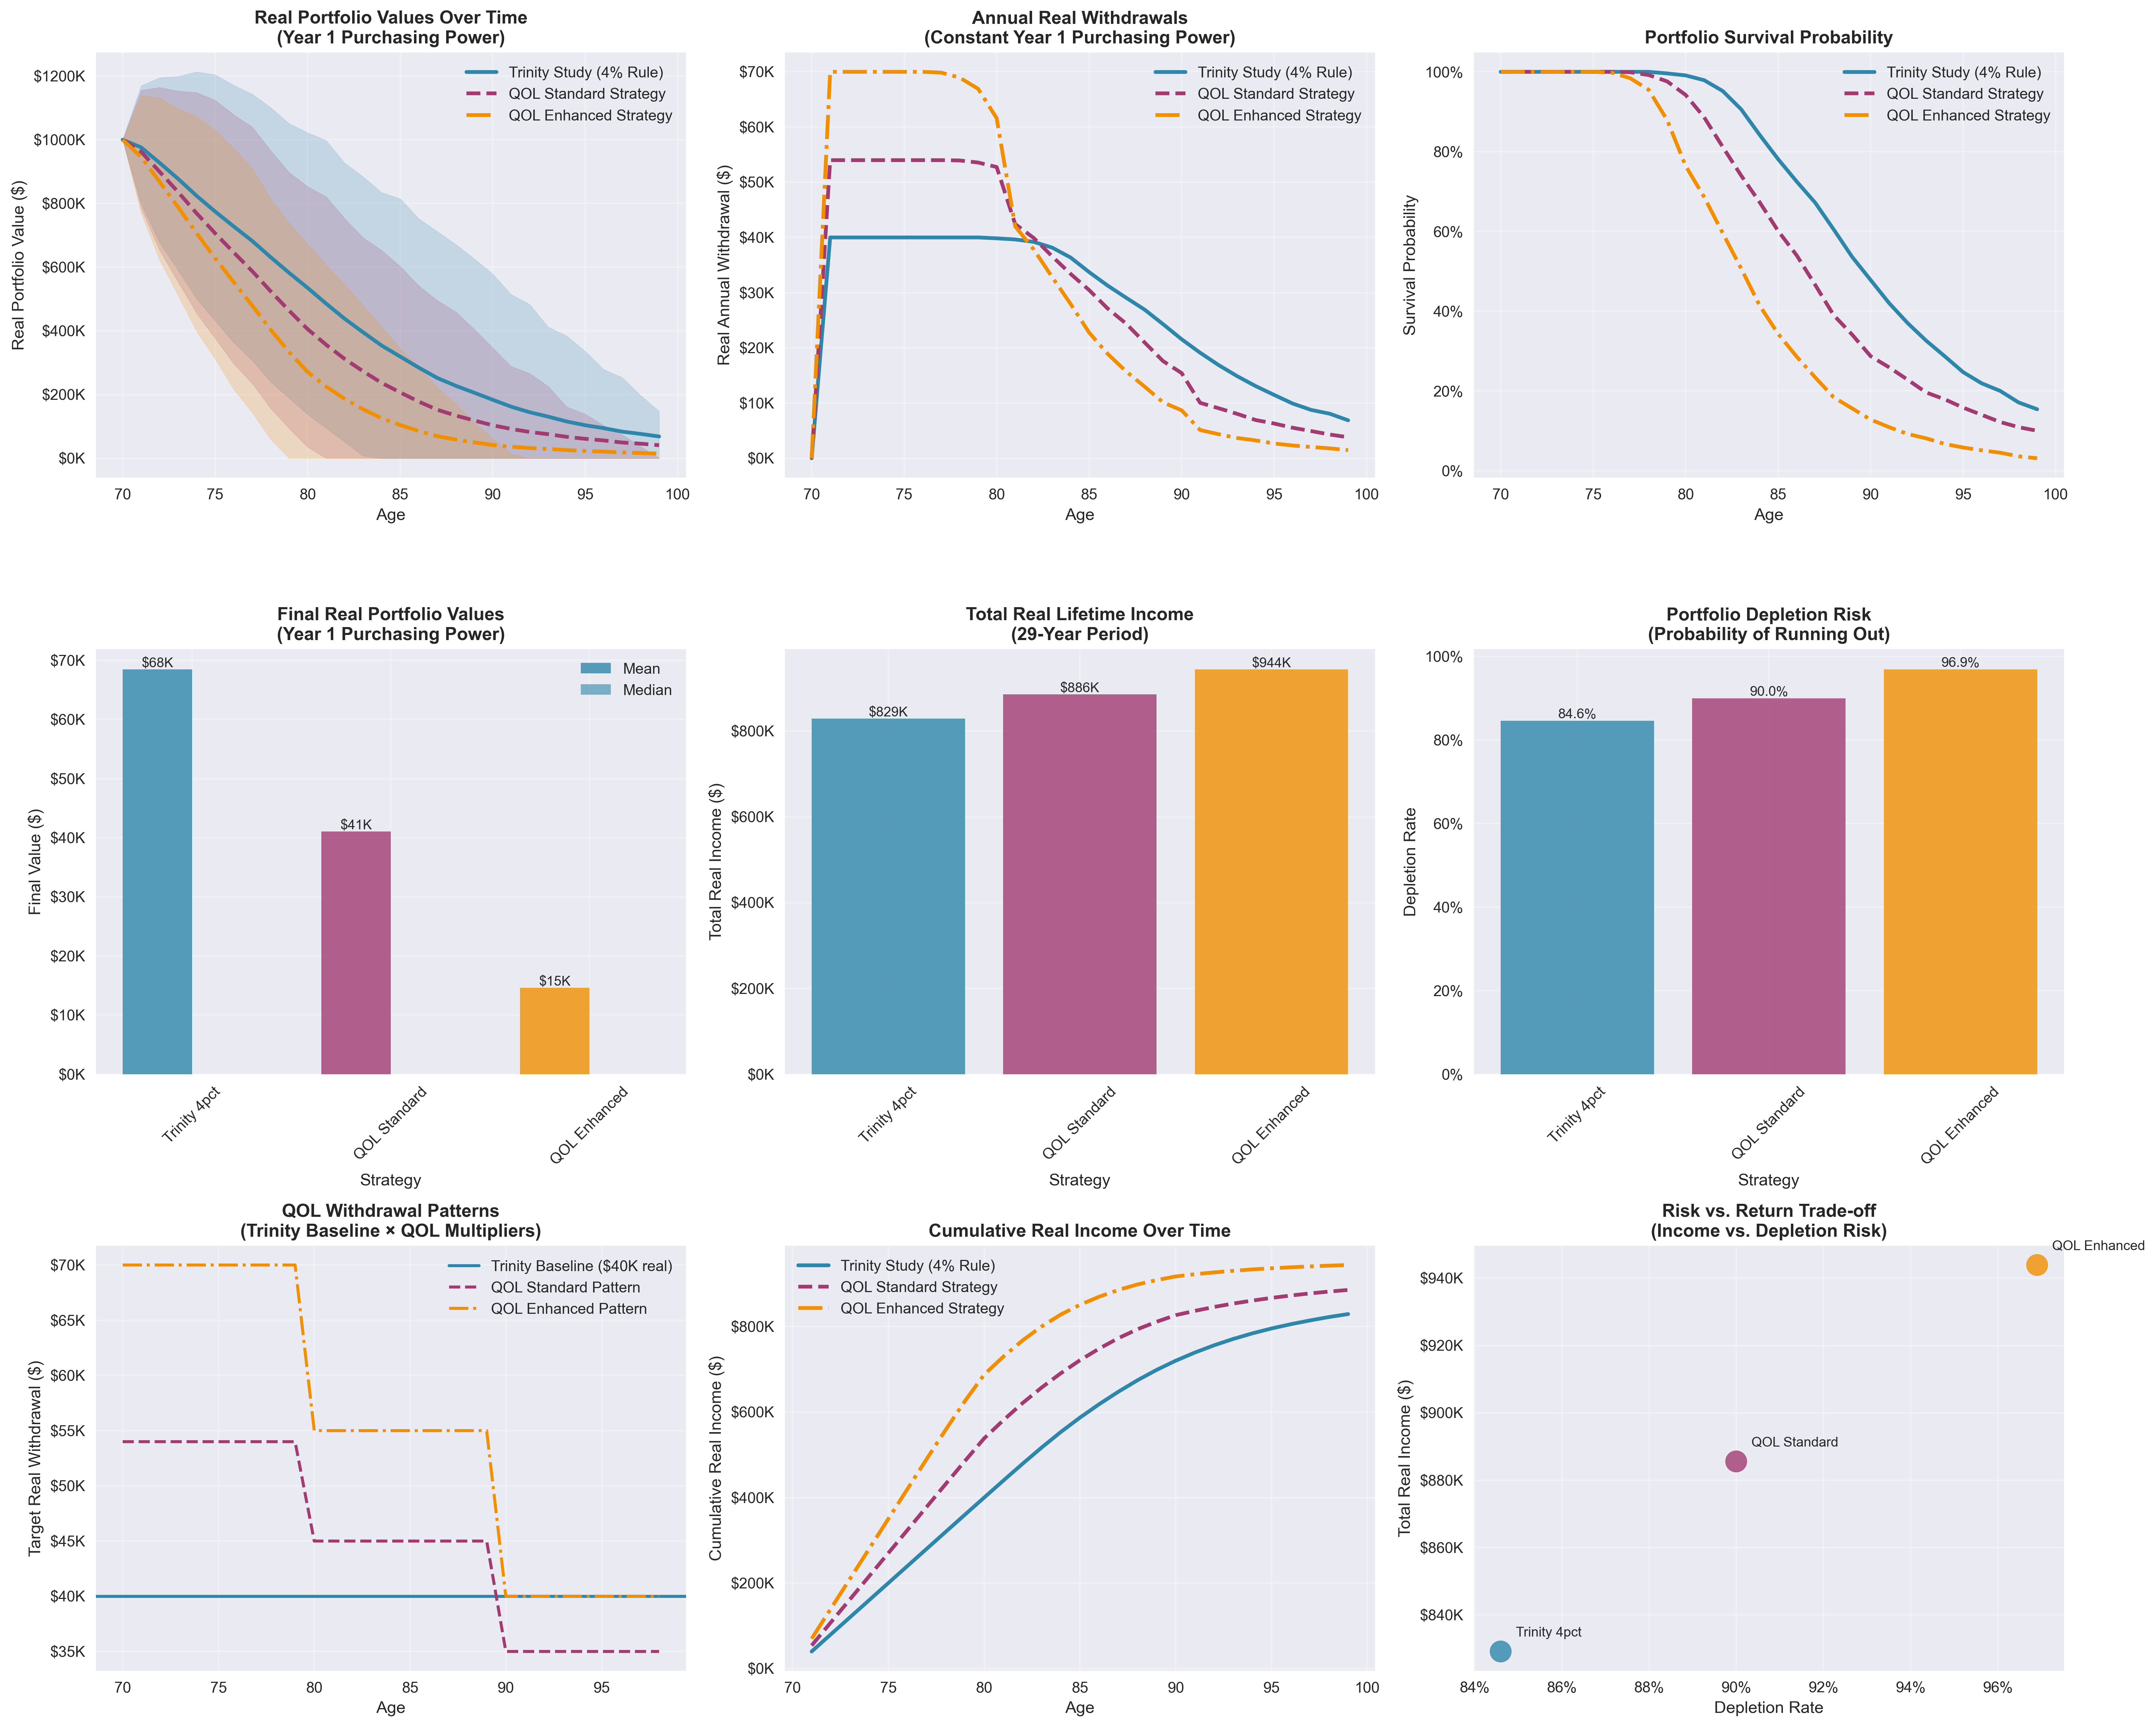
\includegraphics[width=\textwidth]{../charts/comprehensive_qol_analysis.png}
\caption{Comprehensive QOL Framework Analysis - Nine-panel visualization showing portfolio evolution, withdrawal patterns, risk metrics, and strategic trade-offs}
\end{figure}

\section{Decision Framework}

\subsection{Choose Trinity Study If:}
\begin{itemize}
    \item Portfolio preservation is the primary concern
    \item Steady, predictable withdrawals are preferred
    \item Lower risk tolerance for portfolio depletion
    \item Legacy/inheritance planning is important
\end{itemize}

\subsection{Choose QOL Framework If:}
\begin{itemize}
    \item Early retirement enjoyment is prioritized
    \item Comfortable with higher portfolio depletion risk
    \item Prefer front-loaded consumption during healthy years
    \item Less concerned about late-life portfolio preservation
\end{itemize}

\section{Limitations and Disclaimers}

\begin{itemize}
    \item Analysis uses Monte Carlo simulation with realistic but hypothetical market assumptions
    \item Past performance does not guarantee future results
    \item Individual circumstances may significantly affect optimal strategy choice
    \item Professional financial advice recommended for personalized retirement planning
    \item Healthcare costs and long-term care needs not explicitly modeled
\end{itemize}

\section{Conclusion}

The corrected QOL framework analysis demonstrates that quality of life considerations can be meaningfully incorporated into retirement withdrawal strategies. However, these benefits come with measurable trade-offs in portfolio longevity and depletion risk.

The choice between Trinity Study and QOL frameworks ultimately depends on individual risk tolerance, lifestyle preferences, and retirement objectives. Both strategies are now mathematically sound and provide valid foundations for retirement planning decisions.

\vspace{1cm}
\hrule
\vspace{0.5cm}
\footnotesize
\textit{This analysis is for educational and research purposes. Consult qualified financial professionals for personalized retirement planning advice.}

\end{document}